\documentclass[a4paper,11pt]{article}
\usepackage[english]{babel}
\usepackage{a4,fullpage} % small margins
\usepackage{graphicx}

\renewcommand{\familydefault}{\sfdefault} % sans serif font


\title{Knowledge Systems - Assignment 2: Configuration}

\author{Laurens Bronwasser\\
1363956\\
lmbronwa@cs.vu.nl
\and
Martijn Vermaat\\
1362917\\
mvermaat@cs.vu.nl}

\date{March 2005}


\begin{document}


\maketitle


%\renewcommand{\abstractname}{Introduction} % abuse abstract environment
%\begin{abstract}
%  Hmmm... (we kunnen misschien ook zonder intro, gewoon abstract
%  deel weghalen)
%\end{abstract}


\tableofcontents


\section{Knowledge About Components}


\subsection*{Components to Choose From}

\begin{itemize}
\item Tent 
\item Hotel guide 
\item Sleeping bag 
\item Aerobed 
\item Sleeping carpet 
\item Cooking construction
\item Cooking pan
\item Barbeque
\item Trousers
\item Socks
\item Phone
\item PDA
\item Battery charger
\item ...
\end{itemize}

\paragraph{Properties}

To pack the bag in such way that everything fits and that the maximum wait is 
not exceeded, the dimensional and weight properties of every part is recorded in
the component model. The weight is in Kilograms, the dimensions in centimeters.

\begin{itemize}
\item Tent: Weight=12; Dim=10,15,30
\item Hotel guide: Weight=0,12; Dim=12,3,15
\item Sleeping bag: Weight=0,7; Dim=30,25,45
\item Aerobed: Weight=4; Dim=35,30,4
\item Sleeping carpet: Weight=5; Dim=40,25,65
\item Cooking construction: Weight 4,5; Dim=25,20,35
\item Socks: Weight=0,03; Dim=2,6,15
\item ...
\end{itemize}


\subsection*{Component Functions}

\begin{description}

\item{A place to sleep}

Provided by a tent or by a hotel guide.

\item{Something to prepare food}

Provided by a cooking construction and by a barbeque.

\item{Something to sleep on}

Provided by an aerobed and by a sleeping carpet.

\item{Means of communication}

Provided by a phone and by a PDA.

\end{description}


\subsection*{Component Evaluations}

Sleeping in a tent is prefered over sleeping in a hotel
when one goes on a `camping' holiday. But eating healthy
food by using a cooking pan is prefered over using the
barbeque every day. An expensive PDA is likely to be stolen
on a camping. therefore we prefer to take our phone.

This evaluation gives rise to the following evaluation
relationships:

\begin{itemize}
\item Tent $>$ Hotel guide
\item Cooking construction $>$ Barbeque
\item Phone $>$ PDA
\end{itemize}

For other alternatives, we take the smallest one and after
that the one with less weight.


\subsection*{Component Relations}

\paragraph{Required Components}

The components required by other parts can be infered from the abstraction 
hierarchy in figure~\ref{figuur:RequiredComponents}.

\begin{figure}
\begin{center}
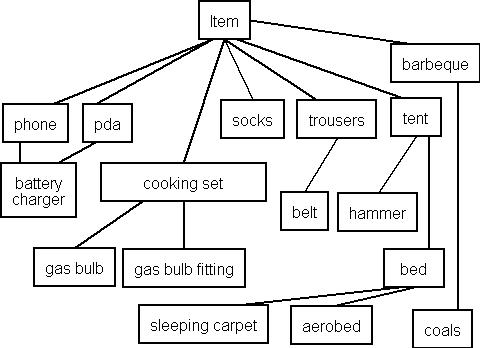
\includegraphics{subcomponents.jpg}
\end{center}
\caption{Required components}
\label{figuur:RequiredComponents}
\end{figure}

\paragraph{Incompatible Components}

\begin{itemize}
\item Hotel guide $\Leftrightarrow$ Tent
\end{itemize}

\paragraph{Alternative Components}

\begin{itemize}
\item Cooking contruction $\Leftrightarrow$ Barbeque
\item Phone $\Leftrightarrow$ PDA
\end{itemize}


\section{Knowledge About Configuration}

We can only take a total of 10 kilograms in our backpack.
Also, the components have to fit in the packpack.
The arrangement model therefore specifies the dimensions of the bag. 
Components with any of their three dimensions longer than the largest dimension 
of the bag will be excluded beforehand.


\section{Knowledge About Sharing}

With the MCF1 technique, we assume there is no sharing of functionality by
several components. This is of course a simplification, because, for example, a
hotel guide could also be used as a note book if we needed one. However, by
using MCF1, we ignore such knowledge about sharing.


\section{Possible Scenario}

The following is part of a possible scenario of applying the
MCF1 technique.

\paragraph{Functional Requirements}

To go on a camping holiday, we need to arrange for the following
in our backpack: something to prepare food, a place to sleep, and
a means of communication.

\paragraph{Key Components}

From these functional requirements we pick our key components. For
the first one, something to prepare food, we can choose between a
barbeque and a cooking construction. However, our evaluation
function says we prefer eating cooked food over eating barbequed
food, so we choose the cooking construction.

For the second requirement, a place to sleep, we can choose between
a tent and a hotel guide. Of course, we prefer sleeping in a tent,
so we take the tent.

As for the third requirement, our evaluation function says we prefer
to take our phone rather than our PDA. As these are exactly the two
components that provide a means of communication, we take our phone.

\paragraph{Required Components}

The cooking construction we choose requires a cooking pan to go
with it. So we add the cooking pan to our configuration. The tent
requires something to sleep on, which can be either an aerobed or
a sleeping carpet, but we prefer the aerobed because it takes less
space (and it sleeps much better too!). For our phone, we need a
battery charger.

\paragraph{Arranging Components}

Now we have satisfied all functional requirements and dependencies,
we try to arrange the choosen components to form a configuration. We
check if the configuration meets the arrangement requirements, such
as total weight and dimensions. If not, we go back, change some
alternatives, and try again.


\end{document}
